\begin{figure}[htbp]
\centering
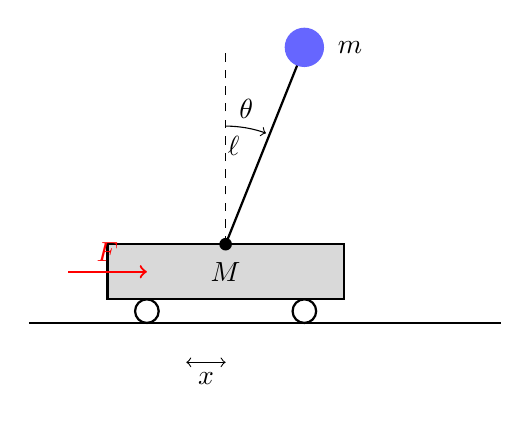
\begin{tikzpicture}
    % Ground
    \draw[thick] (-2,0) -- (4,0);

    % Cart
    \draw[thick, fill=gray!30] (-1,0.3) rectangle (2,1);
    \node at (0.5,0.65) {$M$};

    % Wheels
    \draw[thick, fill=white] (-0.5,0.15) circle (0.15);
    \draw[thick, fill=white] (1.5,0.15) circle (0.15);

    % Pivot
    \fill (0.5,1) circle (0.08);

    % Pendulum rod
    \draw[thick] (0.5,1) -- (1.5,3.5);

    % Pendulum mass
    \fill[blue!60] (1.5,3.5) circle (0.25);
    \node[right] at (1.8,3.5) {$m$};

    % Angle
    \draw[dashed] (0.5,1) -- (0.5,3.5);
    \draw[->] (0.5,2.5) arc (90:70:1.5) node[midway, above] {$\theta$};

    % Length
    \node[left] at (0.8,2.25) {$\ell$};

    % Force
    \draw[->, thick, red] (-1.5,0.65) -- (-0.5,0.65) node[above, midway] {$F$};

    % Position
    \draw[<->] (0,-0.5) -- (0.5,-0.5) node[midway, below] {$x$};
\end{tikzpicture}
\caption{Inverted pendulum on cart.}
\label{fig:inverted_pendulum}
\end{figure}
